\documentclass[11pt, answers]{exam}
\usepackage[utf8]{inputenc}
\usepackage{settings}
% Title
\title{Project 1: Report}
\author{Justin Baker, Eric Brown, Trent DeGiovanni,\\ Edward Gu, Rebecca Hardenbrook}
\date{\today}

\begin{document}
\maketitle

Consider training the following regularized logistic regression model
$$\min_x F(x):= f(x)+\lambda R(x)$$
where
$$f(x)=\frac{1}{2n}\sum^n_{i=1}\log(1+\exp(-b_ia_i^Tx)),$$

with $n$ being the sample size and $a_i\in\R^d$ ($d=50$) is the training data,
$b_i\in\{-1,1\}$ be the label of $a_i$. 
Here, we consider two different regularization functions 
i.e. $\ell_1$-regularization ($R(x)=\lone{x}$) 
and $\ell_2$-regularization ($R(x)=\ltwo{x}^2$).


Please use the code in the zip file to generate 1000 data-label pairs $\{a_i,b_i\}^{1000}_{i=1}.$

\begin{questions}

	\question Derive $\prox{\lambda\lone{x}}{f(x)}$ and $\prox{\lambda\ltwo{x}}{f(x)}$.

	\begin{solution}

		By definition
		$$\prox{\lambda h(x)}{f(x)}=\argmin_v\{h(v)+\frac{1}{2\lambda}\ltwo{x-v}^2\}$$
		Let $h(x)=\lone{x}$
		$$\prox{\lambda \lone{x}}{f(x)}=\argmin_v\{\lone{v}+\frac{1}{2\lambda}\ltwo{x-v}^2\}$$

		With insight we anticipate that the optimum of mixed $\ell_1-\ell_2$ norms is given by the soft-threshold or shrinkage operator.

		For this problem we can use an extension of the optimality conditions to sub-differentiable functions.

		\begin{align*}
		0\in \partial_v F &= \partial_v [\lone{v} +\frac{1}{2\lambda}\ltwo{v-x}^2]\\
		0\in \partial_v F &= \partial_v \lone{v} +\frac{1}{2\lambda}\partial_v \ltwo{v-x}^2\\
		0\in \partial_v F &= \partial_v \lone{v} +\frac{1}{2\lambda}\nabla \ltwo{v-x}^2\\
		0&\in  \lambda \partial_v \lone{v} +v-x
		\end{align*}

		Now we consider the sub-differential for $\ell_1$ component wise.

		$$\partial_v \lone{v} = \begin{cases} \sign{v_i} &\text{for }v_i\neq 0 \\
				[-1,1] & \text{for } v_i=0\end{cases}$$

		Analyzing both cases we have the following.

		$$\begin{cases}0=v_i^*-x+\lambda\sign{v_i^*} & v_i\neq 0\\
			0\in x+\lambda[-1,1] & v_i= 0
		\end{cases}$$

		Solving for the minimizer $v^*$ in terms of $x$.
		$$\begin{cases}v_i^*=x-\lambda\sign{v_i^*} & v_i\neq 0\\
			x\in\lambda[-1,1] & v_i= 0
		\end{cases}$$

		From the first condition we see that if $v_i^*\leq 0$ then $x\leq 0$ (notice that $\lambda>0$).
		$$0>v^* = x+\lambda$$
		Similarly for $v^*>0$ the $x>0$.
		$$0<v^* = x-\lambda$$

		Now using the fact that $x$ and $v^*$ have similar signs we may write the solution for $v^*$
		exclusively in terms of $x$.
		$$v_i = \begin{cases}0 & x\in [-\lambda, \lambda]\\
			x-\lambda\sign{x} & \text{otherwise}
		\end{cases}$$

		This is exactly the shrinkage operator we anticipated to find.

		\vspace{.5in}\hrule\vspace{.5in}

		Now consider $\prox{\lambda\ltwo{x}}{x}$

		Again by definition

		$$\prox{\lambda h(x)}{f(x)}=\argmin_v\{h(v)+\frac{1}{2\lambda}\ltwo{x-v}^2\}$$
		Let $h(x)=\ltwo{x}$
		$$\prox{\lambda \ltwo{x}}{f(x)}=\argmin_v\{\ltwo{v}+\frac{1}{2\lambda}\ltwo{x-v}^2\}$$

		In this instance the function is differentiable everywhere.

		\begin{align*}
		0&= \nabla [\ltwo{v} +\frac{1}{2\lambda}\ltwo{v-x}^2]\\
		0&= \nabla \ltwo{v} +\frac{1}{2\lambda}\nabla \ltwo{v-x}^2\\
		0&= \frac{1}{2}v+\frac{1}{\lambda}v-x\\
		(\frac{1}{2}+\lambda^{-1})v &= \lambda^{-1} x\\
		v &= \frac{2}{2+\lambda}x
		\end{align*}

		Thus the optimal value is given by $v^* = \frac{2}{2+\lambda}x$.

	\end{solution}
	
	\pagebreak
	
	\question For $\lambda=0.001$, numerically solve the problem $\min_xF(x)$ using sub-gradient method,
	proximal gradient method, accelerated proximal gradient method with heavy-ball momentum and Nesterov's
	acceleration.
	Plot $F(x^k)-F(x^*)$ over the iteration $k$ for each method,
	where $x^*$ is in the code that used to generate the training data.
	
	\begin{solution}
	
		For the optimization problem $F(x)=f(x)+\lambda R(x)$
		we implement the following iterative scheme for subgradient descent.
		$$ x_{t+1}=x_t -\eta_t\partial F$$
		
		In the case that $R(x)=\ltwo{x}^2$, the function is everywhere differentiable
		and we have the following
		\begin{align*}
		x_{t+1}&=x_t-\eta_t\partial F(x_t)\\
		x_{t+1}&=x_t-\eta_t\nabla F(x_t)\\
		x_{t+1}&=x_t-\eta_t\bigg[\nabla\frac{1}{2n}\sum^n_{i=1}\log(1+\exp(-b_ia_i^Tx_t)) 
				+ \lambda\nabla \ltwo{x_t}^2\bigg]\\
		x_{t+1}&=x_t-\eta_t\bigg[\frac{1}{2n}\sum^n_{i=1}\frac{-b_ia_i\exp(-b_ia_i^Tx_t)}
				{1+\exp(-b_ia_i^Tx_t)} + 2 \lambda x_t\bigg]
		\end{align*}
		
		In the case that $R(x)=\lone{x}^2$, the function is not differentiable everywhere
		thus we break the subgradient into cases component wise.
		\begin{align*}
		x_{t+1}&=x_t-\eta_t\partial F(x_t)\\
		x_{t+1}&=x_t-\eta_t\bigg[\nabla \frac{1}{2n}\sum^n_{i=1}
				\log(1+\exp(-b_ia_i^Tx_t)) +\lambda\partial \lone{x_t}\bigg]\\
		x_{t+1}&=x_t-\eta_t\bigg[\frac{1}{2n}\sum^n_{i=1}\frac{-b_ia_i\exp(-b_ia_i^Tx_t)}
				{1+\exp(-b_ia_i^Tx_t)} +\lambda \sign{x_i}\bigg]
		\end{align*}
		
		As we showed in class we expect that the subgradient with stepsize $\eta_t \approx \frac{1}{\sqrt{t}}$ has a sublinear convergence rate of $\mathcal{O}(\frac{1}{\sqrt{t}})$. This is what we observe in the following plot.
		
		\begin{figure}[H]
		\centering
		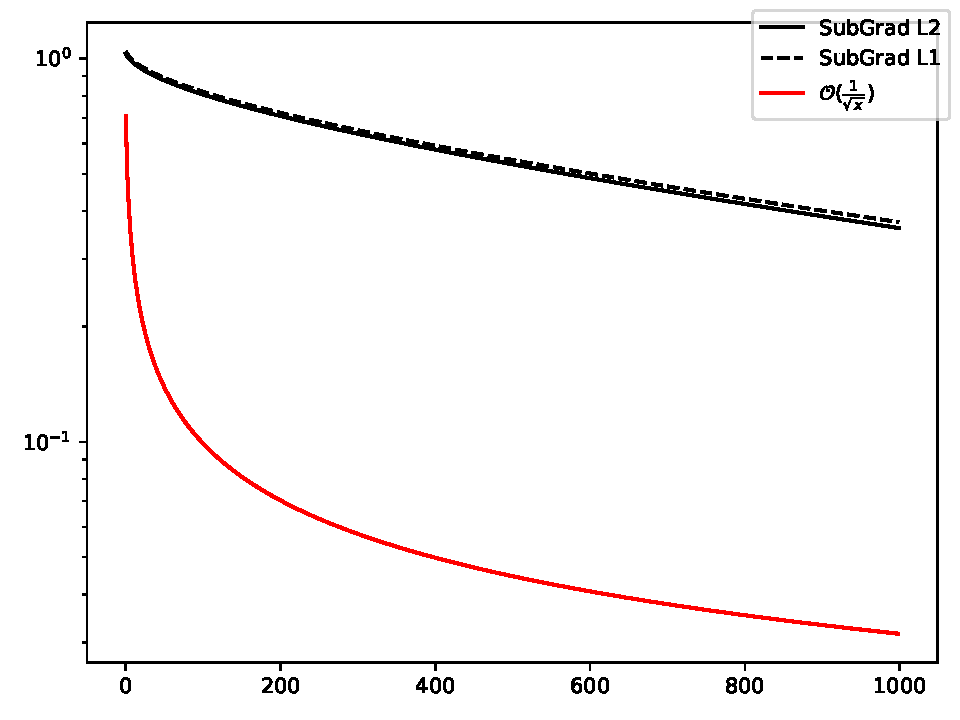
\includegraphics[width=.75\textwidth]{../out/SubGrad.pdf}
		\caption{Order of Subgradient Method}
		\end{figure}
		
		\vspace{.5in}\hrule\vspace{.5in}

		For the optimization problem $F(x)=f(x)+\lambda h(x)$
		we implement the following iterative scheme for proximal gradient descent.
		$$ x_{t+1}=\prox{\lambda h(x)}{x_t -\eta_t\partial f}$$
		
		In the case that $h(x)=\ltwo{x}$, the proximal function is everywhere differentiable.
		For simplicity let $h(x)=\ltwo{x}^2$ and $\lambda=2$.
		\begin{align*}
			x_{t+1}&=\prox{\lambda h(x)}{x_t -\eta_t\partial f}\\
			x_{t+1}&=\argmin_v\{\ltwo{v-x_t +\eta_t\partial f}^2+\frac{\lambda}{2} \ltwo{v}^2\\
			0&=v^*-x_t +\eta_t\partial f+\lambda v^*\\
			v* &= \frac{x_t-\eta_t\partial f}{1+\lambda}\\
			x_{t+1}&=v^* = \frac{x_t-\eta_t\partial f}{1+\lambda}
		\end{align*}
		
				In the case that $h(x)=\lone{x}$, the proximal function is not differentiable everywhere.
				Therefore we must consider the function in cases.
		\begin{align*}
			x_{t+1}&=\prox{\lambda h(x)}{x_t -\eta_t\partial f}\\
			x_{t+1}&=\argmin_v\{\ltwo{v-x_t +\eta_t\partial f}^2+\lambda \lone{v}
		\end{align*}	
		
		In part 1 we showed that the solution to this problem is the soft-threshold algorithm
		
		\begin{align*}
			x = \begin{cases}0 & x_i-\eta_t\nabla f(x)_i\in [-\lambda, \lambda]\\
			x_i-\eta\nabla f(x)_i-\lambda\sign{x_i-\eta_t\nabla f(x)_i} & \text{otherwise}
		\end{cases}
		\end{align*}
		
		If $f(x)+h(x)$ is $L$-smooth and $\eta_t\equiv 1/L$ then we can anticipate that the method is order $\mathcal{O}(\frac{1}{t})$.
		This is not the case for $h(x)=\lone{x}$, however it is true for $h(x)=\ltwo{x}^2$. 
		Additionally (as we will see later) the value of lambda will force the $\lone{x}$ regularization term to dominate after a certain number of iterations and the value of $x^*$ will become zero.
		
		\begin{figure}[H]
		\centering
		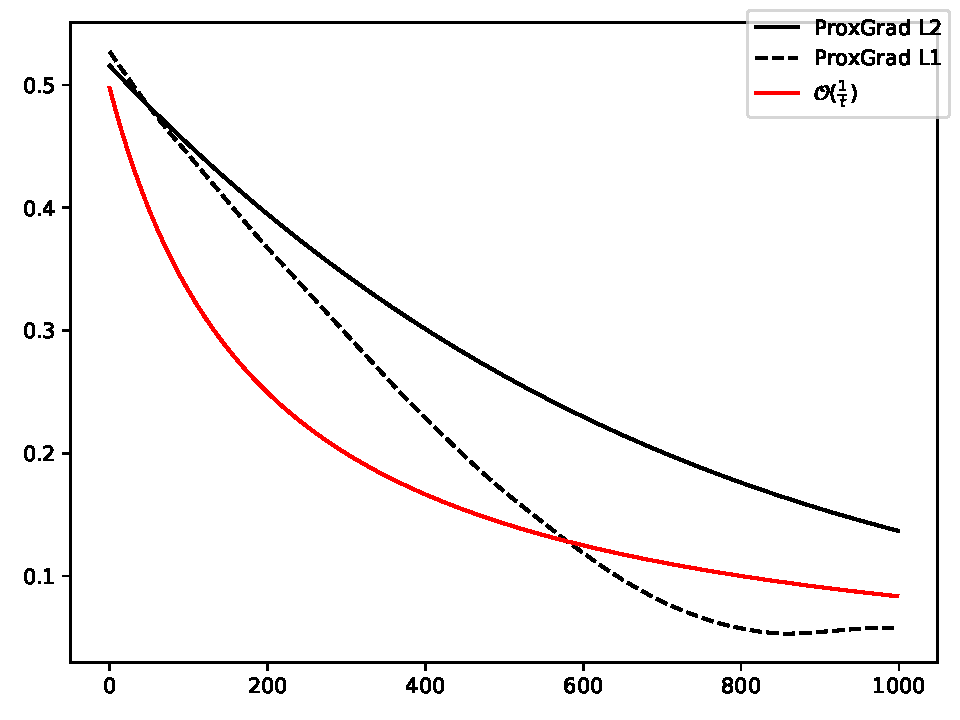
\includegraphics[width=.75\textwidth]{../out/ProxGrad.pdf}
		\caption{Order of Proximal Gradient Method}
		\end{figure}
		
		\vspace{.5in}\hrule\vspace{.5in}
		
		For the optimization problem $F(x)=f(x)+\lambda h(x)$
		we implement the following iterative scheme for momentum proximal gradient descent.
		$$ x_{t+1}=\prox{\lambda h(x)}{x_t -\eta_t\partial f + \theta(x_t-x_{t-1})}$$
		
		In the case that $h(x)=\ltwo{x}$, the proximal function is everywhere differentiable. Similar to the case above we find the following iterative scheme.
		$$x_{t+1}=\frac{x_t-\eta_t\partial f+\theta(x_t-x_{t-1})}{1+\lambda}$$
		
		Similarly if $h(x)=\lone{x}$, the proximal function has similar analysis to the non-accelerated case.
		\begin{align*}
			x^{t+1} = \begin{cases}0 & x^t_i-\eta_t\nabla f(x^t)_i+\theta_t(x^t_i-x^{t-1}_i)\in [-\lambda, \lambda]\\
			x^t_i-\eta\nabla f(x^t)_i-&\\
			\quad-\lambda\sign{x^t_i-\eta_t\nabla f(x^t)_i+\theta_t(x^t_i-x^{t-1}_i)} & \text{otherwise}
		\end{cases}
		\end{align*}	
		
		If $f(x)+h(x)$ is $L$-smooth and $\eta_t\equiv 1/L$ then we can anticipate that the method is order $\mathcal{O}(\frac{1}{(t+1)^2})$.			
		\begin{figure}[H]
		\centering
		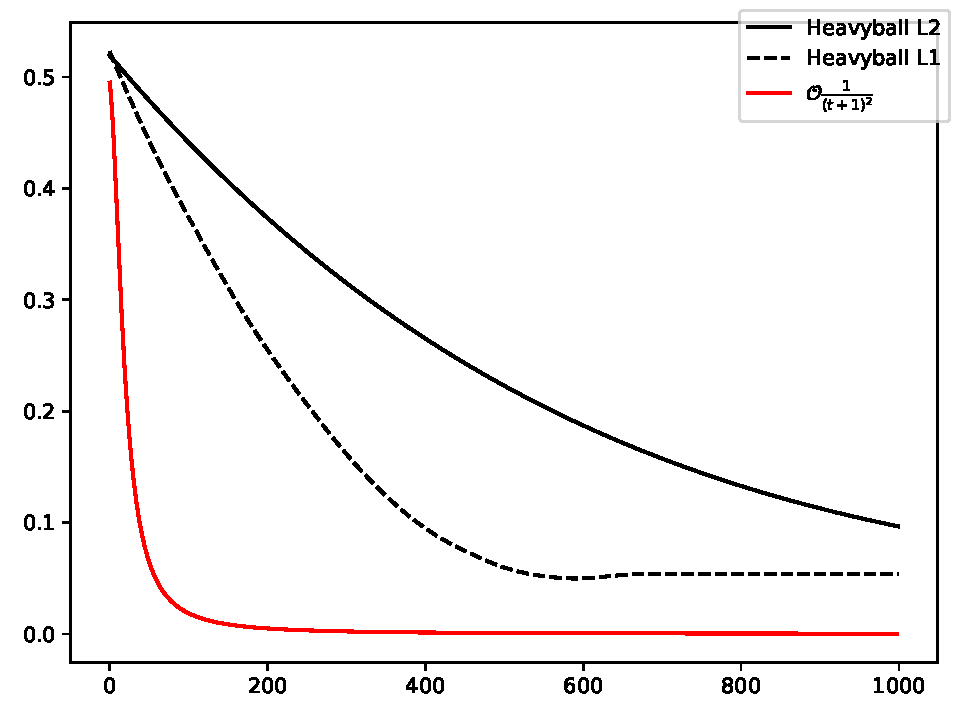
\includegraphics[width=.75\textwidth]{../out/HBGrad.pdf}
		\caption{Order of Momentum Accelerated Proximal Gradient Method}
		\end{figure}
		
		\vspace{.5in}\hrule\vspace{.5in}
		
		Finally for the Nesterov accelerated proximal algorithm we implement the following iterative scheme.
		\begin{align*}
		y_t &= x_t+\frac{t}{t+3}(x_t-x_{t-1})\\
		x_{t+1}&=\prox{\lambda h(x)}{y_t -\eta_t\partial f(y_t)}
		\end{align*}
		
		Although this is not a descent algorithm it can be shown that it maintains $\mathcal{O}(\frac{1}{(t+1)^2})$ convergence for $\eta_t\equiv 1/L$ if $f$ is $L$-smooth.
		\begin{figure}[H]
		\centering
		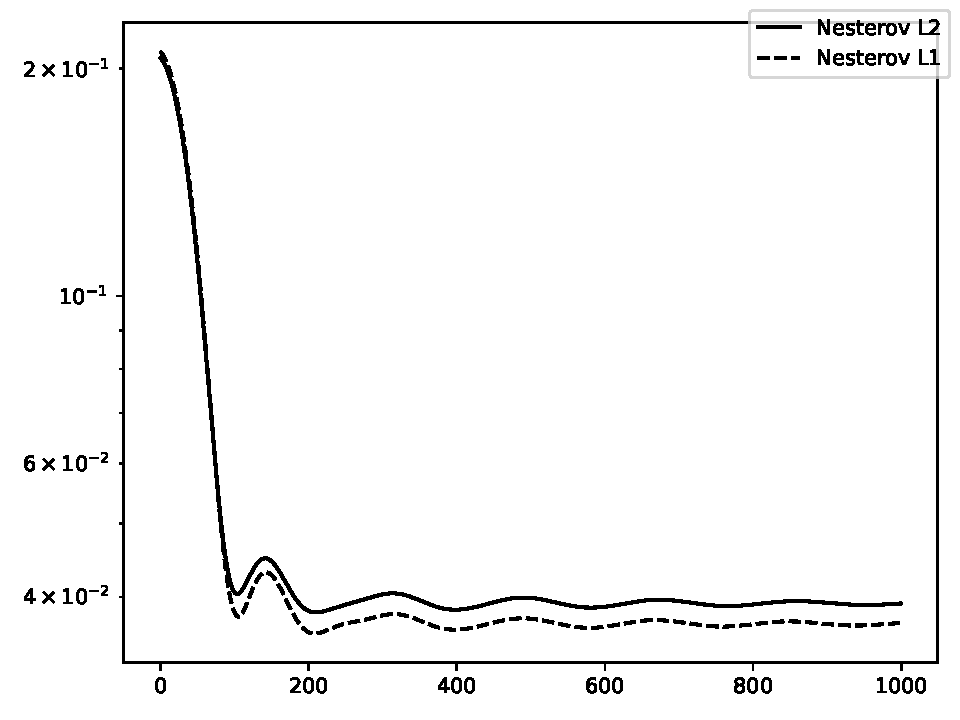
\includegraphics[width=.75\textwidth]{../out/NestGrad.pdf}
		\caption{Nesterov Oscillations}
		\end{figure}
		
		It is important to note here that the minimizer $x^*$ suggested to use in this model is a minimizer of the MLE function $f(x)$ without regularization. Therefore for any nonzero value of $\lambda$ we can anticipate that the true solution is different than $x^*$. Thus explaining why if we compare $F(x)-F(x^*)$ we see the oscillating behavior of the Nesterov acceleration but we do not see the continued convergence pattern.
		
	\end{solution}

	\pagebreak

	\question Test different $\lambda$, e.g. $0.005,0.01,0.05,0.1$ and see how $x^k$ changes after you run enough number of iterations.
	
	\begin{solution}
	
		Consider the coefficients of the logistic regression function. Because of the regularization terms the values of the solution are penalized for being particularly large. For instance the first term of the coefficients is 1. However, when regularizing based on the norm of $x$ values tend towards zero.
		
		 As $\lambda$ increases the values of $x$ tend towards zero. If the regularization term is the $\ell_2$ norm then all values tend towards zero. If the regularization term is the $\ell_1$ norm then all values tend towards zero.
		 
		\begin{figure}[H]
		\centering
		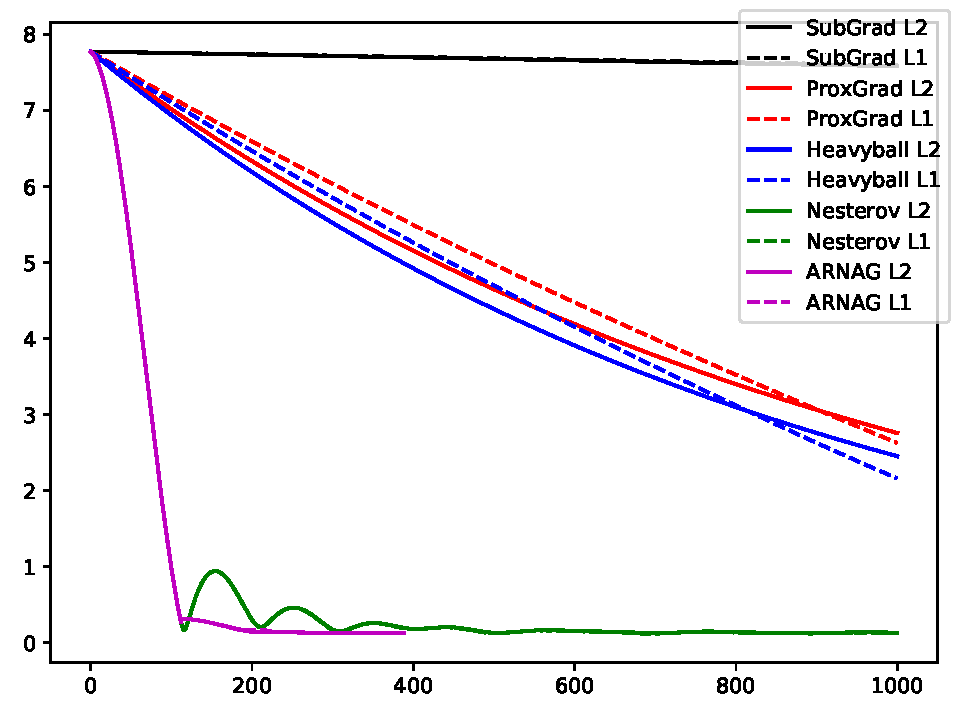
\includegraphics[width=.75\textwidth]{../out/001xl2.pdf}
		\caption{L2 Norm of $x^*$ using $R(x)=\ltwo{x},\lambda=0.001$}
		\end{figure}
		\begin{figure}[H]
		\centering
		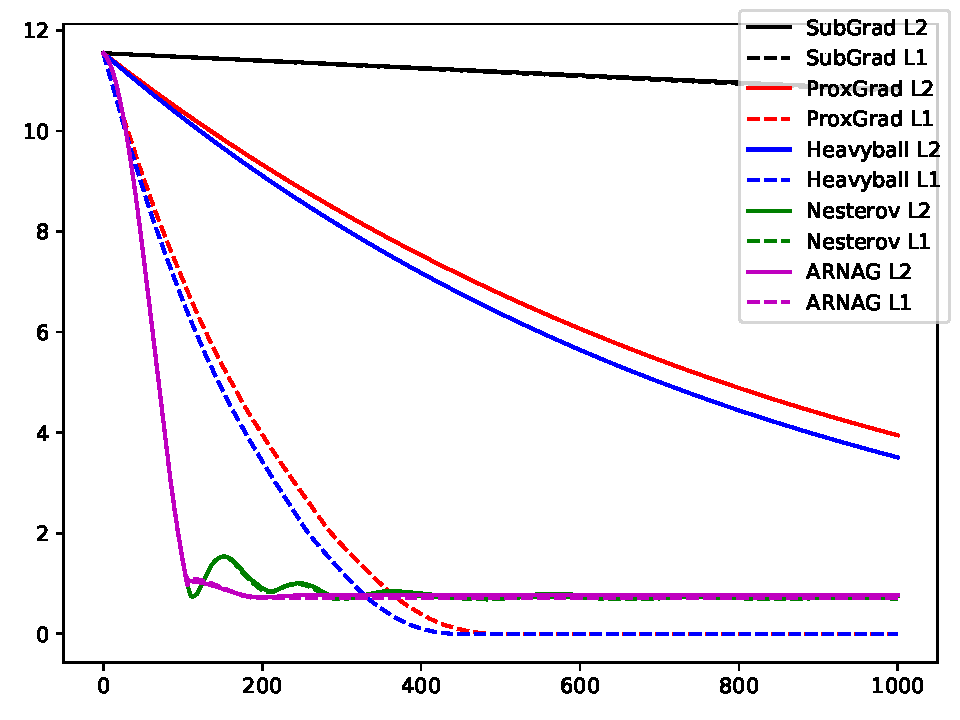
\includegraphics[width=.75\textwidth]{../out/001xl1.pdf}
		\caption{L1 Norm of $x^*$ using $R(x)=\lone{x},\lambda=0.001$}
		\end{figure}
		
		In the above figures the norm of $x^*$ approaches zero much more slowly than in the following figures.
		This corresponds to larger $\lambda$ penalizing the value of $x^*$ more heavily.
		For a full set of figures please see the appendix.
		\begin{figure}[H]
		\centering
		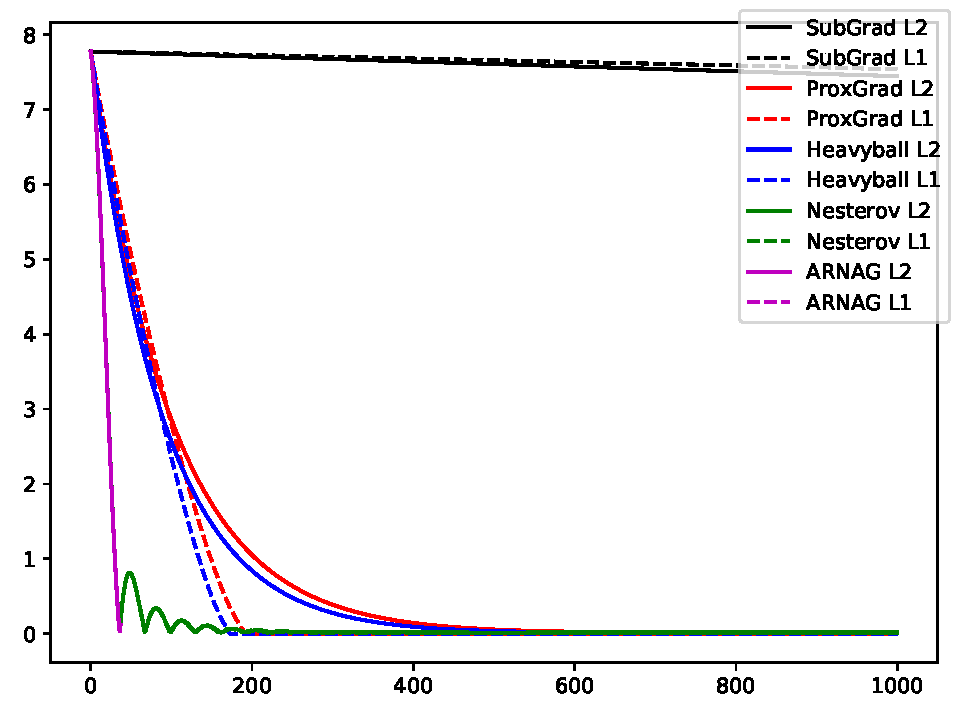
\includegraphics[width=.75\textwidth]{../out/01xl2.pdf}
		\caption{L2 Norm of $x^*$ using $R(x)=\ltwo{x},\lambda=0.01$}
		\end{figure}
		\begin{figure}[H]
		\centering
		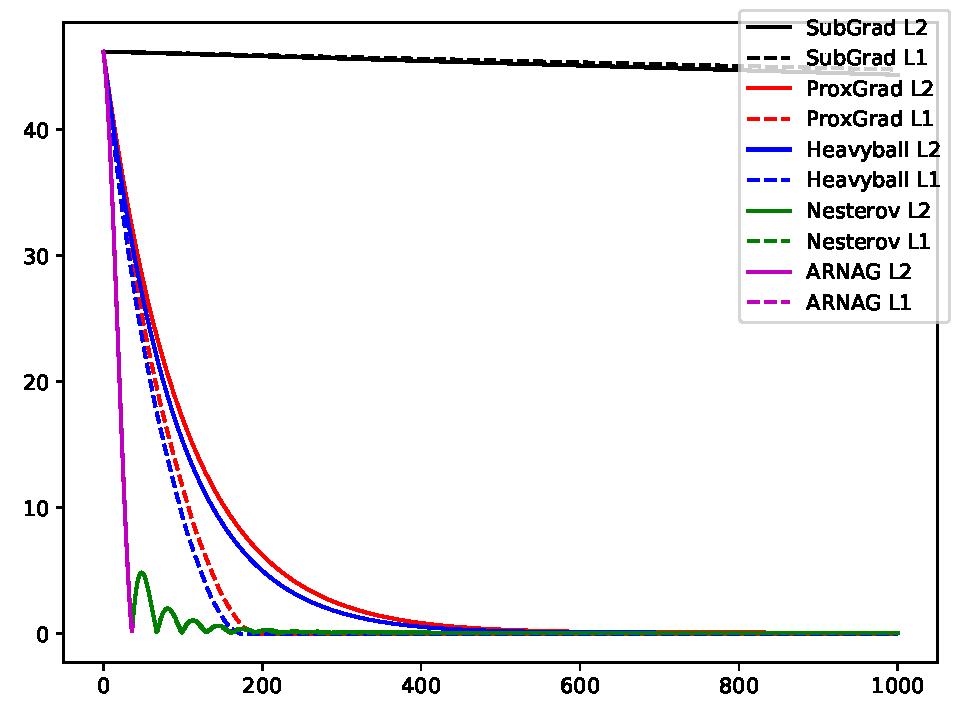
\includegraphics[width=.75\textwidth]{../out/01xl1.pdf}
		\caption{L1 Norm of $x^*$ using $R(x)=\lone{x},\lambda=0.01$}
		\end{figure}
	\end{solution}
	
	\pagebreak

	\question Can you propose any approach to further accelerate the training process?
	
	\begin{solution}
	
	One way to improve the methods is to use adaptive restart in Nesterov accelerated proximal gradient. This idea follows that from ``Sharpness, Restart and Acceleration" by Roulet and d'Aspremont (NeurIPs 2017). Because the Nesterov accelerated gradient is not a descent algorithm, it may suffer when $\frac{t}{t+3}\sim 1$. Therefore, if $\nabla f (x_t-x_{t-1})<0$ we reset the value of $t$ to zero. This is shown to have linear convergence if $f$ is $L$-smooth.
	
	Although the problem described above hides the true performance of the methods, in the figure below you can see that the adaptive restart performs better than standard Nestorov. Additionally, it does not have oscillations as Nestorov does.
	
		\begin{figure}[H]
		\centering
		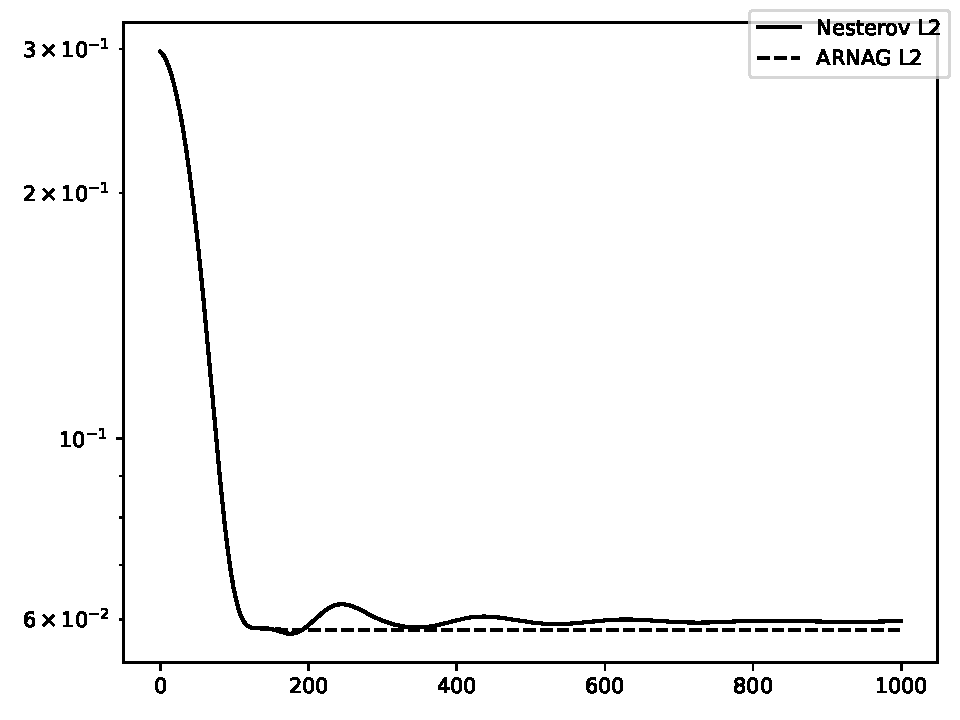
\includegraphics[width=.75\textwidth]{../out/ARNAG.pdf}
		\caption{Adaptive Restart of Nestorov Accelerated Gradient}
		\end{figure}
	
	
	Comparing all of these methods together we have the following figure.
	
		\begin{figure}[H]
		\centering
		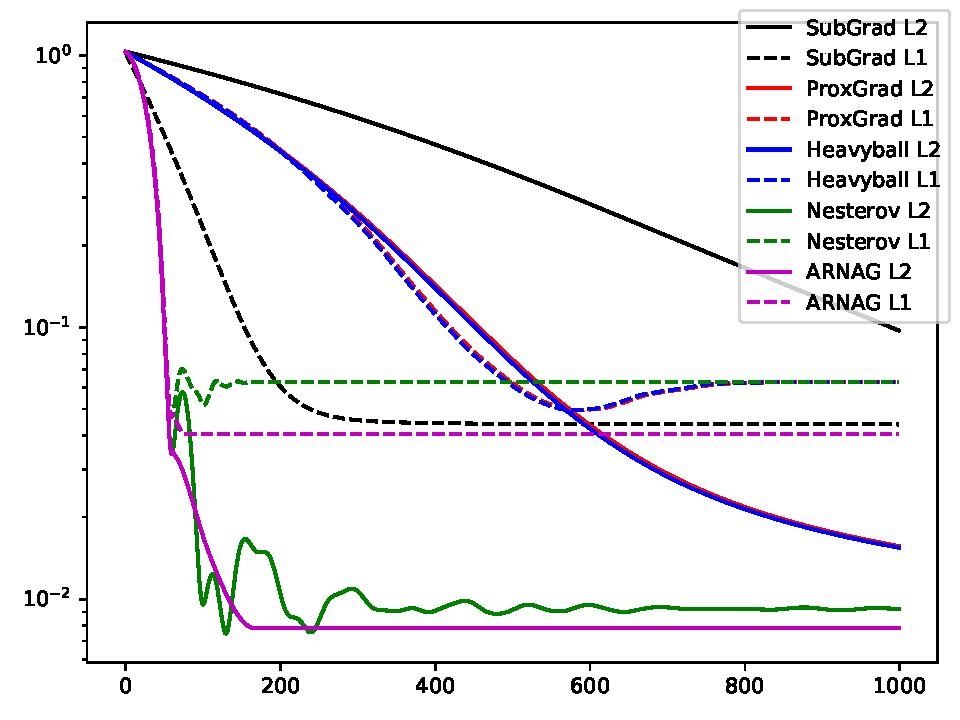
\includegraphics[width=.75\textwidth]{../out/error.pdf}
		\caption{Comparison of all methods}
		\end{figure}
	\end{solution}


\end{questions}

\pagebreak

\appendix
\section{Appendix}
		\begin{figure}[H]
		\centering
		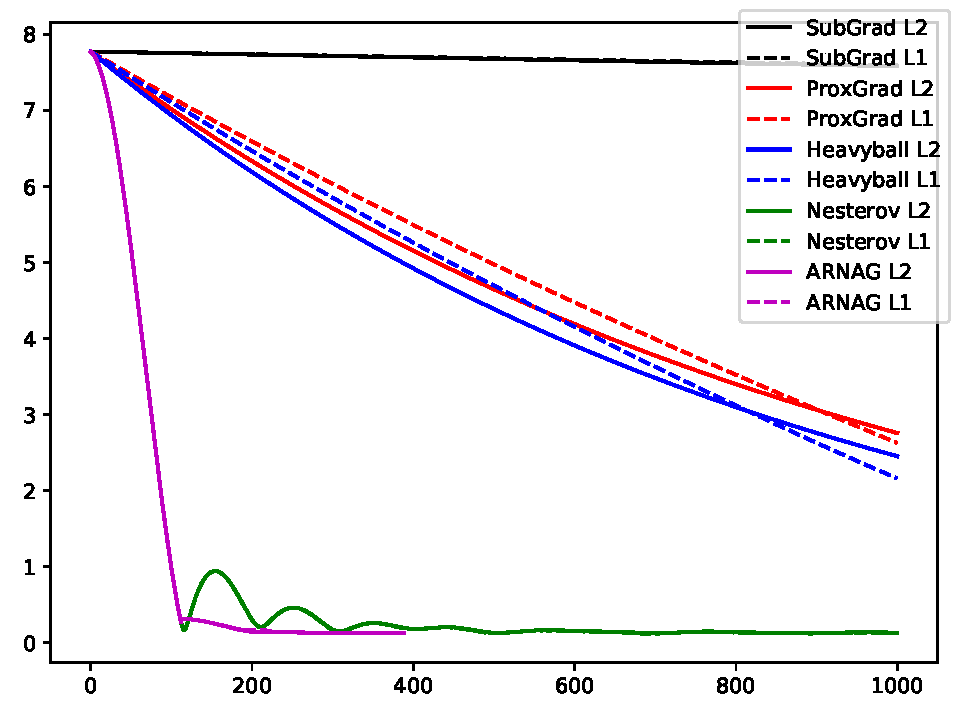
\includegraphics[width=.75\textwidth]{../out/001xl2.pdf}
		\caption{L2 Norm of $x^*$ using $R(x)=\ltwo{x},\lambda=0.001$}
		\end{figure}
		\begin{figure}[H]
		\centering
		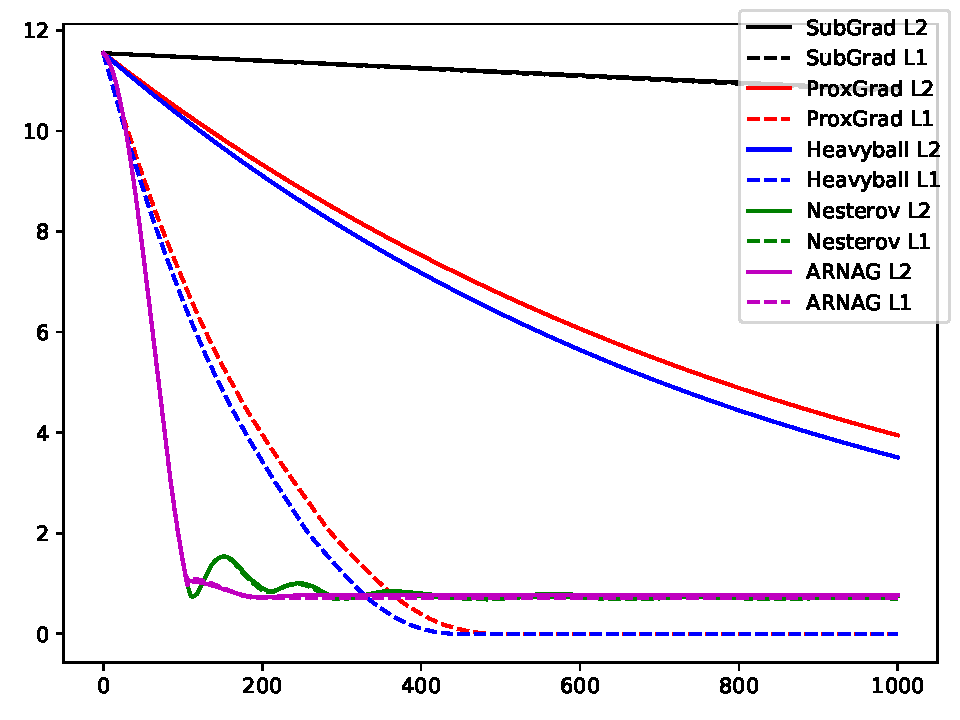
\includegraphics[width=.75\textwidth]{../out/001xl1.pdf}
		\caption{L1 Norm of $x^*$ using $R(x)=\lone{x},\lambda=0.001$}
		\end{figure}		\begin{figure}[H]
		\centering
		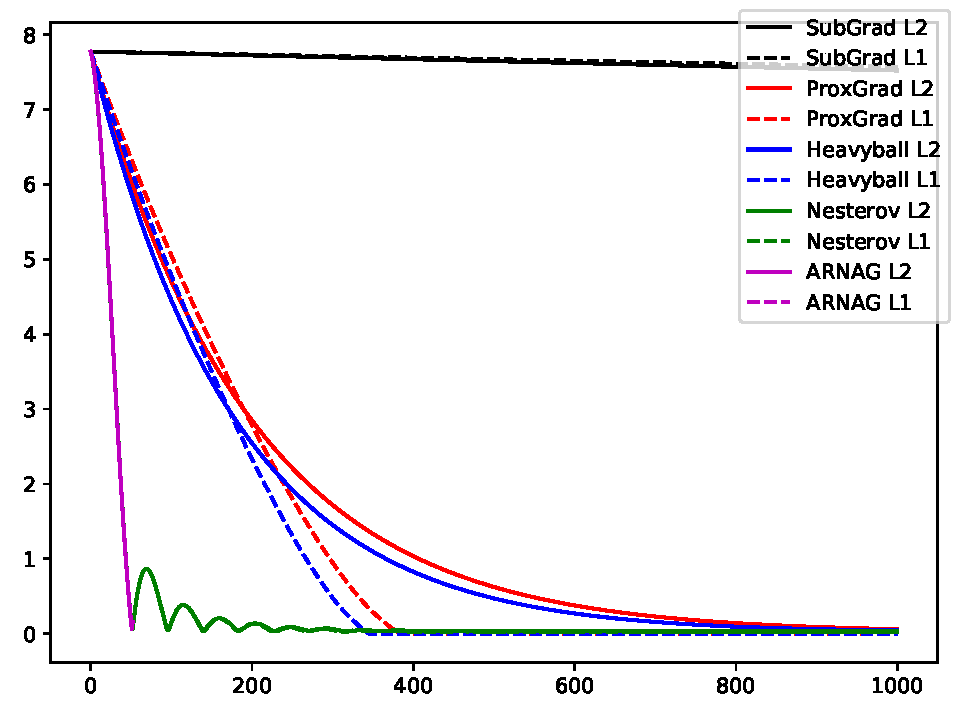
\includegraphics[width=.75\textwidth]{../out/005xl2.pdf}
		\caption{L2 Norm of $x^*$ using $R(x)=\ltwo{x},\lambda=0.005$}
		\end{figure}
		\begin{figure}[H]
		\centering
		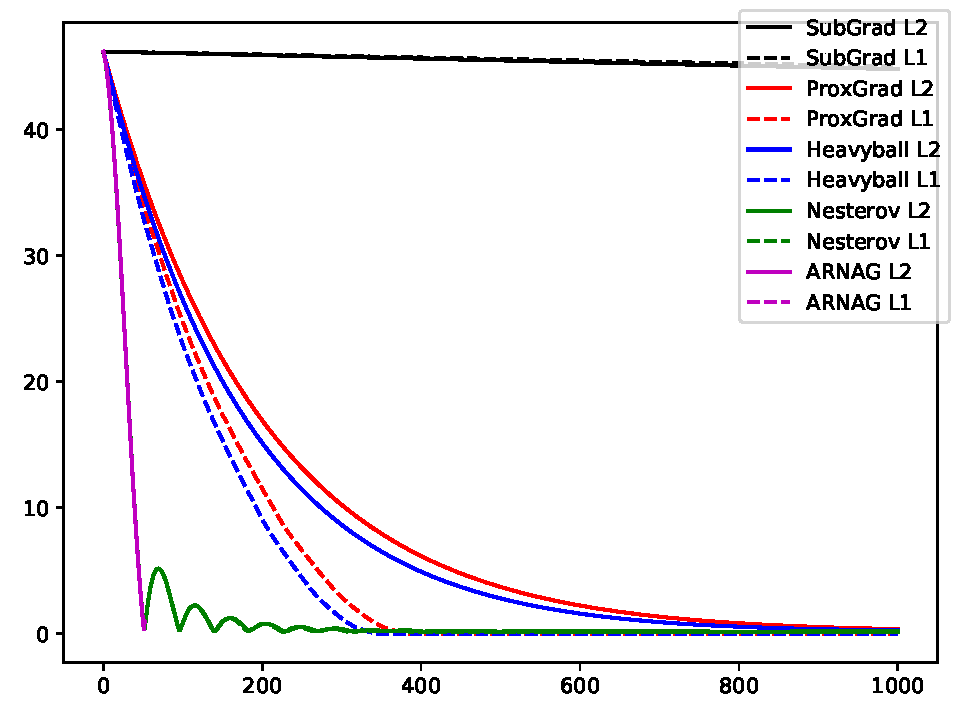
\includegraphics[width=.75\textwidth]{../out/005xl1.pdf}
		\caption{L1 Norm of $x^*$ using $R(x)=\lone{x},\lambda=0.005$}
		\end{figure}		\begin{figure}[H]
		\centering
		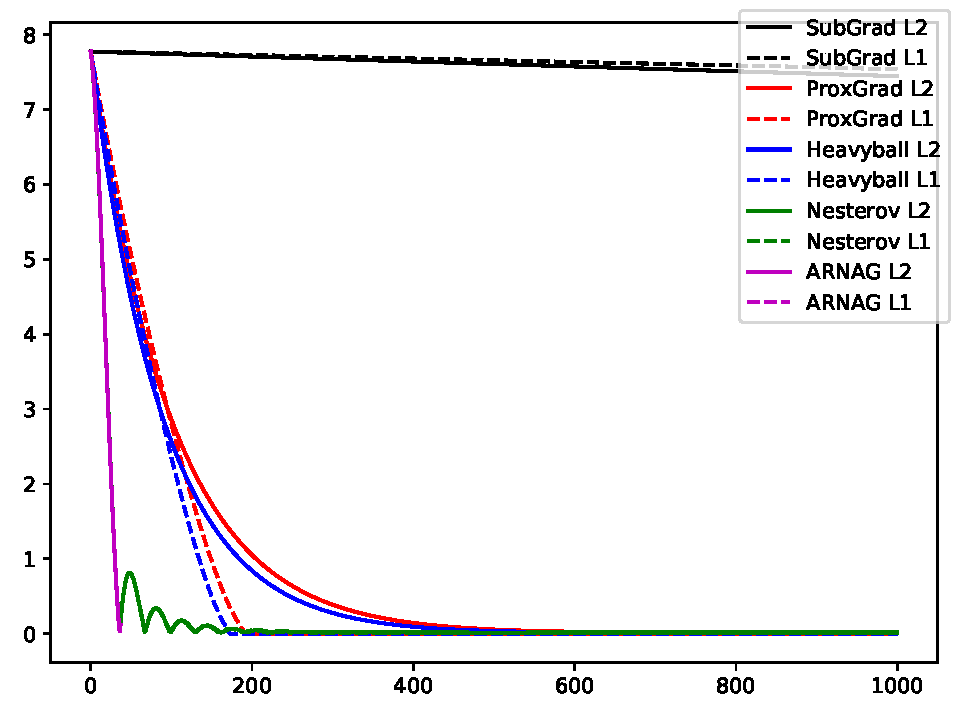
\includegraphics[width=.75\textwidth]{../out/01xl2.pdf}
		\caption{L2 Norm of $x^*$ using $R(x)=\ltwo{x},\lambda=0.01$}
		\end{figure}
		\begin{figure}[H]
		\centering
		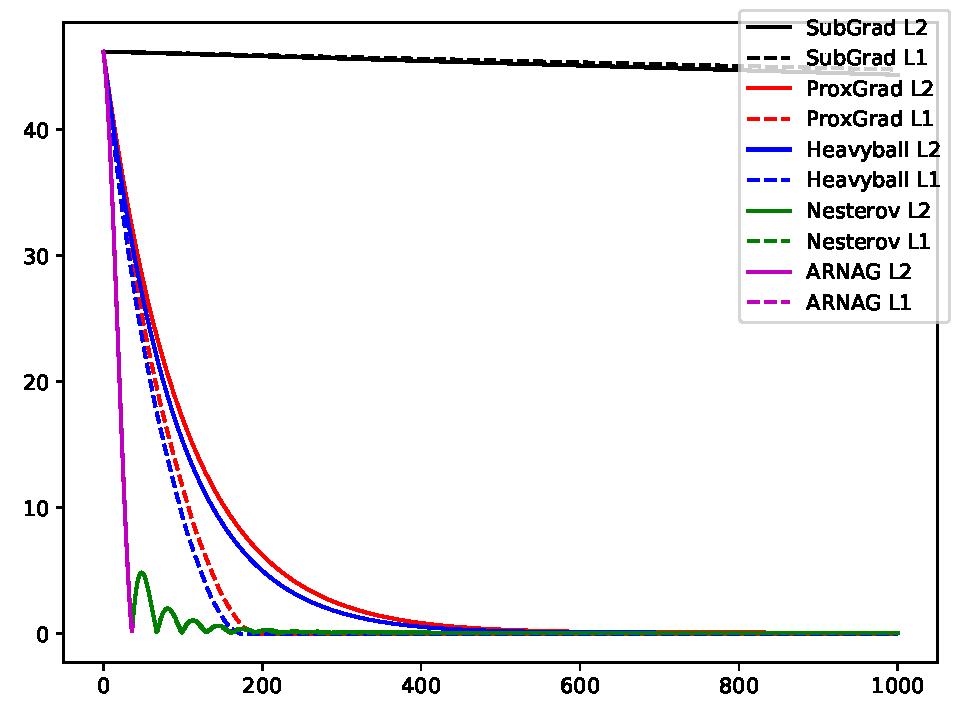
\includegraphics[width=.75\textwidth]{../out/01xl1.pdf}
		\caption{L1 Norm of $x^*$ using $R(x)=\lone{x},\lambda=0.01$}
		\end{figure}		\begin{figure}[H]
		\centering
		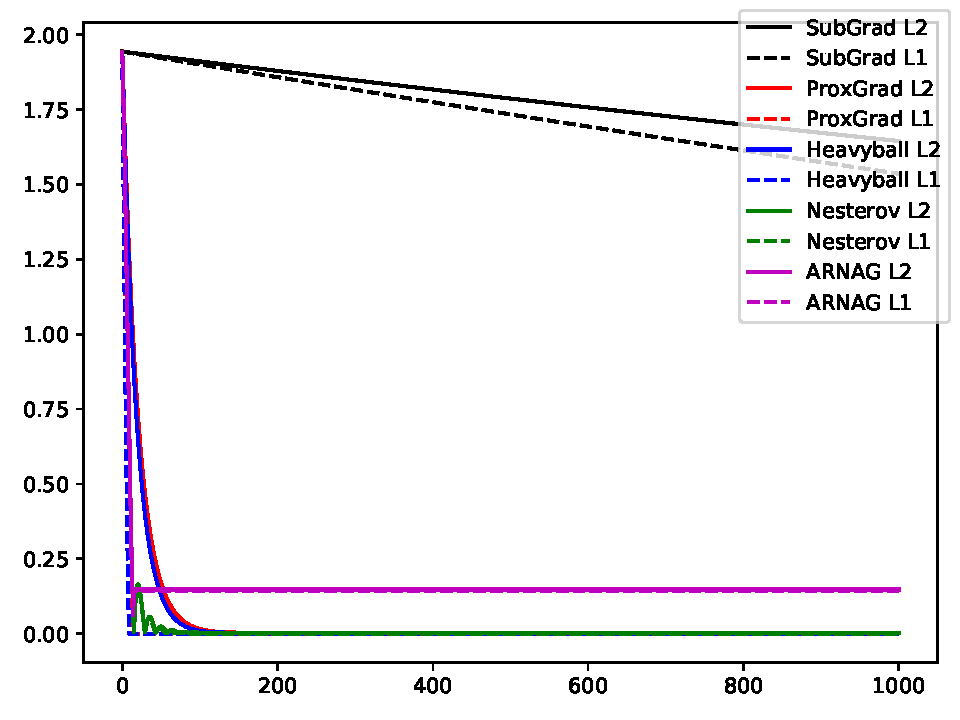
\includegraphics[width=.75\textwidth]{../out/05xl2.pdf}
		\caption{L2 Norm of $x^*$ using $R(x)=\ltwo{x},\lambda=0.05$}
		\end{figure}
		\begin{figure}[H]
		\centering
		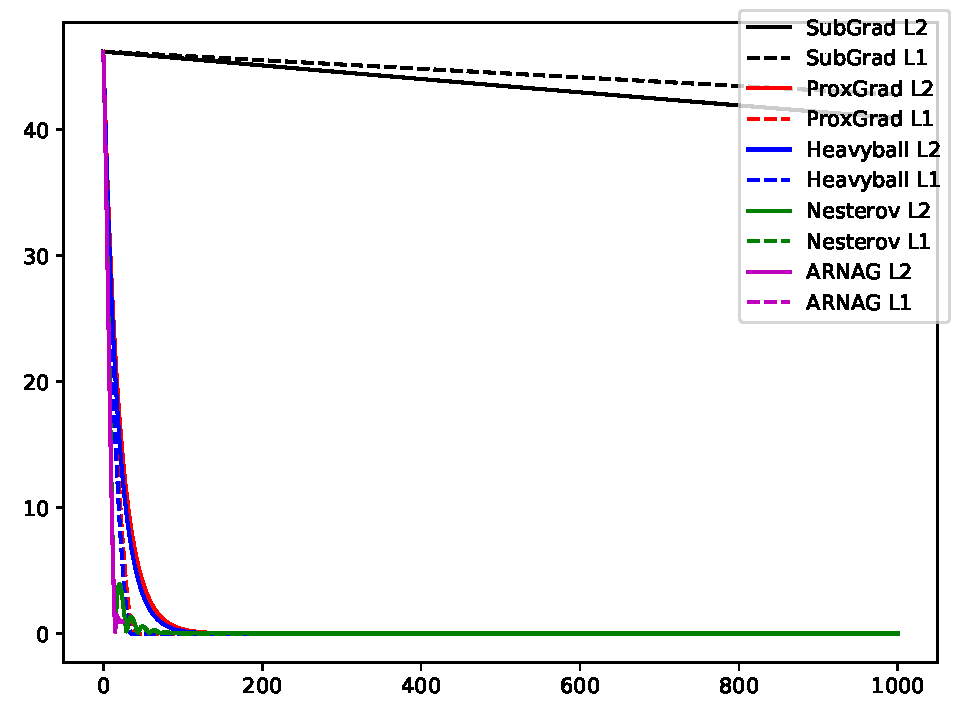
\includegraphics[width=.75\textwidth]{../out/05xl1.pdf}
		\caption{L1 Norm of $x^*$ using $R(x)=\lone{x},\lambda=0.05$}
		\end{figure}		\begin{figure}[H]
		\centering
		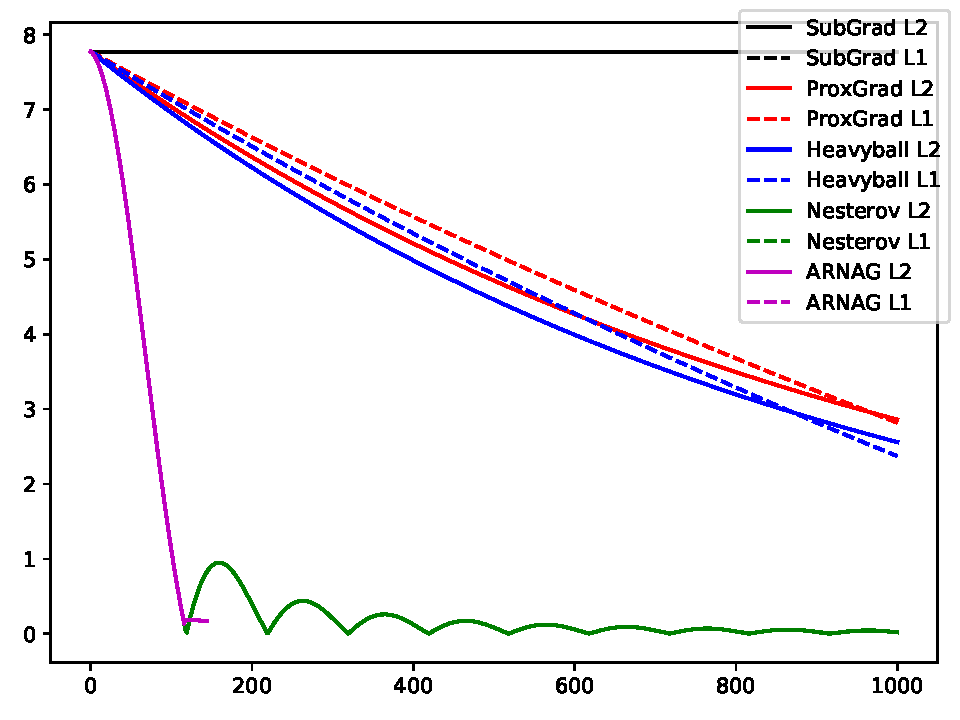
\includegraphics[width=.75\textwidth]{../out/xl2.pdf}
		\caption{L2 Norm of $x^*$ using $R(x)=\ltwo{x},\lambda=0.1$}
		\end{figure}
		\begin{figure}[H]
		\centering
		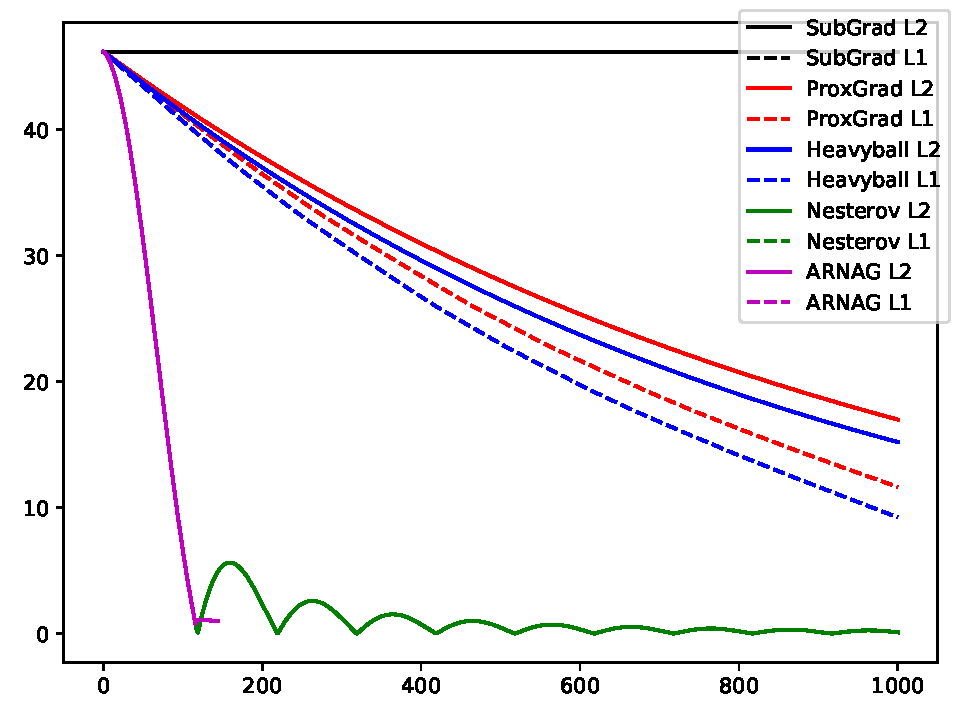
\includegraphics[width=.75\textwidth]{../out/xl1.pdf}
		\caption{L1 Norm of $x^*$ using $R(x)=\lone{x},\lambda=0.1$}
		\end{figure}


\end{document}
